\chapter{Clase 22}

\section{Conservación de la masa}

Sea $V$ un volumen de control fijo, limitado por una superficie cerrada $S$ cuya normal exterior es $\hat n$. La masa contenida en $V$ es
\[
M(t)=\int_V\rho(\vec r,t)\,dV.
\]
La masa solo puede cambiar si cruza la frontera. Como $\rho\vec v\cdot\hat n$ es el flujo másico saliente por unidad de área, la conservación global de la masa se escribe
\[
\oint_S\rho\vec v\cdot\hat n\,dS
=-\frac{dM}{dt}
=-\frac{d}{dt}\int_V\rho\,dV.
\]
El signo menos indica que un flujo saliente positivo disminuye la masa dentro de $V$. Puesto que el volumen de control es fijo, podemos introducir la derivada dentro de la integral:
\[
\oint_S\rho\vec v\cdot\hat n\,dS
=-\int_V\frac{\partial\rho}{\partial t}\,dV.
\]
Aplicamos el teorema de Gauss al miembro izquierdo:
\[
\int_V\nabla\cdot(\rho\vec v)\,dV
=-\int_V\frac{\partial\rho}{\partial t}\,dV,
\]
por lo que
\[
\int_V\left[\frac{\partial\rho}{\partial t}
+\nabla\cdot(\rho\vec v)\right]dV=0.
\]
Como esta igualdad se cumple para cualquier volumen $V$, el integrando debe anularse en cada punto. Obtenemos la forma local de la ecuación de continuidad:
\[
\boxed{\frac{\partial\rho}{\partial t}
+\nabla\cdot(\rho\vec v)=0.}
\]

Para expresar el balance siguiendo el movimiento del fluido, expandimos la divergencia del producto:
\[
\nabla\cdot(\rho\vec v)
=\vec v\cdot\nabla\rho+\rho\,\nabla\cdot\vec v.
\]
Entonces
\[
\frac{\partial\rho}{\partial t}
+\vec v\cdot\nabla\rho
=-\rho\,\nabla\cdot\vec v.
\]
La derivada material de un campo escalar $q$ se define como
\[
\frac{Dq}{Dt}
=\frac{\partial q}{\partial t}+\vec v\cdot\nabla q.
\]
En efecto, si una partícula ocupa la posición $\vec r_p(t)$, entonces $d\vec r_p/dt=\vec v$ y, por la regla de la cadena,
\[
\frac{d}{dt}q(\vec r_p(t),t)
=\frac{\partial q}{\partial t}
+\frac{d\vec r_p}{dt}\cdot\nabla q
=\frac{\partial q}{\partial t}+\vec v\cdot\nabla q
=\frac{Dq}{Dt}.
\]
Por tanto, la continuidad también se escribe
\[
\boxed{\frac{D\rho}{Dt}+\rho\,\nabla\cdot\vec v=0.}
\]
En un fluido incompresible, la densidad de cada partícula material permanece constante, es decir, $D\rho/Dt=0$. Para $\rho\ne0$ resulta
\[
\boxed{\nabla\cdot\vec v=0.}
\]
La divergencia mide precisamente la tasa relativa de cambio del volumen material: si $\delta V$ es un pequeño volumen que se mueve con el fluido,
\[
\frac{1}{\delta V}\frac{D(\delta V)}{Dt}=\nabla\cdot\vec v.
\]
Por ello, para un fluido incompresible esa tasa es cero y el volumen de cada elemento material se conserva.

\section{Ley de Leonardo y velocidad promedio}

Consideremos un tubo de corriente en régimen estacionario. Sus paredes están formadas por líneas de corriente, por lo que la velocidad es tangente a la pared y no hay flujo a través de la superficie lateral. La masa que atraviesa por unidad de tiempo las secciones de entrada y salida debe ser la misma:
\[
\dot m
=\int_{A_1}\rho\vec v\cdot\hat n_1\,dA
=\int_{A_2}\rho\vec v\cdot\hat n_2\,dA,
\]
donde $\hat n_1$ y $\hat n_2$ se eligen en el sentido del flujo. Para densidad constante se cancela $\rho$ y queda el caudal volumétrico
\[
Q=\int_A\vec v\cdot\hat n\,dA.
\]
La misma conclusión se ve integrando $\nabla\cdot\vec v=0$ sobre el volumen del tubo:
\[
0=\oint_S\vec v\cdot\hat n_{\!S}\,dS
=-\int_{A_1}\vec v\cdot\hat n_1\,dA
+\int_{A_2}\vec v\cdot\hat n_2\,dA.
\]
El signo menos aparece porque la normal exterior en la entrada apunta en sentido opuesto al flujo; en la salida apunta en el sentido del flujo. Por tanto,
\[
\int_{A_1}\vec v\cdot\hat n_1\,dA
=\int_{A_2}\vec v\cdot\hat n_2\,dA.
\]

Definimos la rapidez normal promedio en una sección por
\[
\bar v=\frac{1}{A}\int_A\vec v\cdot\hat n\,dA.
\]
Por definición, $Q=A\bar v$. Como $Q$ es el mismo en todas las secciones del tubo,
\[
\boxed{A_1\bar v_1=A_2\bar v_2.}
\]
Esta relación se conoce como \textbf{ley de Leonardo}: en un flujo estacionario e incompresible, la rapidez promedio es inversamente proporcional al área transversal. Para flujo uniforme, la velocidad normal tiene un valor constante $v_0$ en toda la sección y
\[
Q=\int_A v_0\,dA
=v_0\int_A dA
=v_0A.
\]
Si el fluido es compresible, lo que se conserva es el caudal másico, $\rho_1A_1\bar v_1=\rho_2A_2\bar v_2$; el caudal volumétrico no tiene por qué ser constante.

\begin{figure}[H]
\centering
\begin{tikzpicture}[
  >=Latex,
  line cap=round,
  line join=round,
  font=\small,
  pared/.style={draw=blue!65!black, line width=1pt},
  flujo/.style={->, red!75!black, line width=1.1pt}
]
\fill[blue!5]
  (0,1.05) .. controls (1.8,1.05) and (3.7,0.62) .. (6,0.48)
  -- (6,-0.48) .. controls (3.7,-0.62) and (1.8,-1.05) .. (0,-1.05)
  -- cycle;
\draw[pared] (0,1.05) .. controls (1.8,1.05) and (3.7,0.62) .. (6,0.48);
\draw[pared] (0,-1.05) .. controls (1.8,-1.05) and (3.7,-0.62) .. (6,-0.48);
\draw[densely dashed,gray] (0.35,-0.98) -- (0.35,0.98);
\draw[densely dashed,gray] (5.7,-0.50) -- (5.7,0.50);
\node[above] at (0.35,1.08) {$A_1$};
\node[above] at (5.7,0.52) {$A_2$};
\draw[flujo] (0.65,0.35) -- (1.55,0.35);
\draw[flujo] (1.65,-0.1) -- (2.55,-0.1);
\draw[flujo] (3.25,0.18) -- (4.2,0.13);
\draw[flujo] (4.45,-0.16) -- (5.5,-0.15);
\node[below] at (1.1,0.25) {$\bar v_1$};
\node[below] at (4.95,-0.3) {$\bar v_2$};
\draw[thick,orange!85!black] (0.25,0.05)
  .. controls (1.8,0.05) and (2.6,-0.02) .. (3.1,-0.05)
  .. controls (4.1,-0.1) and (4.8,-0.05) .. (5.85,0);
\fill (1.2,0.04) circle (2pt);
\fill (4.8,-0.05) circle (2pt);
\node[above] at (1.2,0.14) {$1$};
\node[above] at (4.8,0.05) {$2$};
\end{tikzpicture}
\par\medskip
\textbf{Figura 35.} Tubo de corriente con dos secciones y una línea de corriente interior. Al reducirse el área, aumenta la rapidez promedio del flujo incompresible; los puntos 1 y 2 están sobre la misma línea de corriente.
\label{fig:clase22-tubo}
\end{figure}

\subsection{Promedio de un perfil de velocidad no uniforme}

Si la rapidez varía sobre una sección, no se puede reemplazar directamente la integral de flujo por el producto de un valor local y el área. Consideremos el perfil axisimétrico de un conducto circular de radio $R$:
\[
v(r)=V_0\left(1-\frac{r}{R}\right)^m,
\qquad 0\le r\le R,\quad m>0,
\]
donde $r$ es la distancia al eje. Un anillo de radio $r$ y espesor $dr$ tiene área diferencial $dA=2\pi r\,dr$, y el área total es $A=\pi R^2$. Entonces
\[
\begin{aligned}
\bar v
&=\frac{1}{A}\int_Av\,dA\\
&=\frac{1}{\pi R^2}\int_0^R
V_0\left(1-\frac{r}{R}\right)^m2\pi r\,dr\\
&=\frac{2V_0}{R^2}\int_0^R
\left(1-\frac{r}{R}\right)^m r\,dr.
\end{aligned}
\]
Para evaluar la integral, hacemos $u=r/R$, de modo que $r=Ru$, $dr=R\,du$ y los límites pasan de $0,R$ a $0,1$:
\[
\begin{aligned}
\int_0^R\left(1-\frac{r}{R}\right)^m r\,dr
&=R^2\int_0^1(1-u)^m u\,du\\
&=R^2\int_0^1(1-s)s^m\,ds
\qquad (s=1-u)\\
&=R^2\left(\int_0^1s^m\,ds-\int_0^1s^{m+1}\,ds\right)\\
&=R^2\left(\frac{1}{m+1}-\frac{1}{m+2}\right)\\
&=\frac{R^2}{(m+1)(m+2)}.
\end{aligned}
\]
Al sustituir el resultado,
\[
\boxed{\bar v=\frac{2V_0}{(m+1)(m+2)}.}
\]
Para $m=\tfrac12$,
\[
\bar v
=\frac{2V_0}{(\tfrac32)(\tfrac52)}
=\frac{8}{15}V_0
\approx0.53V_0.
\]
En el eje, $v(0)=V_0$, el máximo del perfil; en la pared, $v(R)=0$. Por tanto, la rapidez promedio sobre la sección es menor que la rapidez local en el centro.

\begin{figure}[H]
\centering
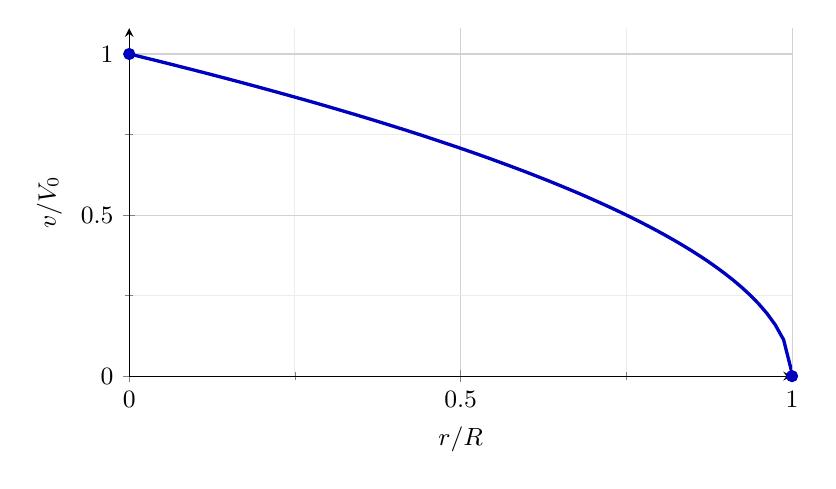
\begin{tikzpicture}
\begin{axis}[
  width=10cm,
  height=6cm,
  xmin=0, xmax=1,
  ymin=0, ymax=1.08,
  xlabel={$r/R$},
  ylabel={$v/V_0$},
  xtick={0,0.5,1},
  ytick={0,0.5,1},
  grid=both,
  major grid style={gray!35},
  minor tick num=1,
  minor grid style={gray!15},
  axis lines=left,
  tick label style={font=\small},
  label style={font=\small}
]
\addplot[blue!75!black, very thick, domain=0:1, samples=80] {(1-x)^0.5};
\addplot[only marks, mark=*, mark size=2pt, blue!75!black] coordinates {(0,1) (1,0)};
\end{axis}
\end{tikzpicture}
\par\medskip
\textbf{Figura 36.} Perfil $v(r)=V_0(1-r/R)^{1/2}$ en un conducto circular. La rapidez es máxima en el eje y se anula en la pared; el promedio sobre la sección es $8V_0/15$.
\end{figure}

\section{Balance de momento y ecuación de Euler}

La ecuación de Cauchy expresa la conservación local del momento lineal. Para un volumen de control fijo $V$, el balance integral es
\[
\frac{d}{dt}\int_V\rho\vec v\,dV
=-\oint_S\rho\vec v(\vec v\cdot\hat n)\,dS
+\oint_S\boldsymbol{\sigma}\cdot\hat n\,dS
+\int_V\vec f\,dV,
\]
donde $\vec f$ es la fuerza de cuerpo por unidad de volumen y $\boldsymbol{\sigma}\cdot\hat n$ es la tracción. El primer término del miembro derecho representa el momento que sale por transporte; los otros dos son las fuerzas de contacto y de cuerpo. Como $V$ es fijo, llevamos la derivada temporal al integrando y aplicamos el teorema de Gauss a los flujos:
\[
\int_V\left[\frac{\partial(\rho v_i)}{\partial t}+\partial_j(\rho v_i v_j)\right]dV
=\int_V\left[f_i+\partial_j\sigma_{ij}\right]dV.
\]
Al ser $V$ arbitrario, los integrandos deben ser iguales en cada punto. Así se obtiene, componente a componente,
\[
\frac{\partial(\rho v_i)}{\partial t}
+\partial_j(\rho v_i v_j)
=f_i+\partial_j\sigma_{ij}.
\]
Aquí $\partial_j=\partial/\partial x_j$, se suma sobre el índice repetido $j$ e $i$ identifica la componente de momento. Expandimos el lado izquierdo:
\[
\begin{aligned}
\frac{\partial(\rho v_i)}{\partial t}
+\partial_j(\rho v_i v_j)
&=\rho\frac{\partial v_i}{\partial t}
+v_i\frac{\partial\rho}{\partial t}
+\rho v_j\partial_jv_i
+v_i\partial_j(\rho v_j)\\
&=\rho\left(\frac{\partial v_i}{\partial t}
+v_j\partial_jv_i\right)
+v_i\left[\frac{\partial\rho}{\partial t}
+\partial_j(\rho v_j)\right].
\end{aligned}
\]
El término entre corchetes se anula por continuidad. Además,
\[
\frac{Dv_i}{Dt}
=\frac{\partial v_i}{\partial t}+v_j\partial_jv_i,
\qquad
\frac{D\vec v}{Dt}
=\frac{\partial\vec v}{\partial t}
+(\vec v\cdot\nabla)\vec v.
\]
Así se obtiene la forma local de Cauchy:
\[
\boxed{\rho\frac{D\vec v}{Dt}
=\vec f+\vec\nabla\cdot\boldsymbol{\sigma}^{\,T}.}
\]
Con la convención tensorial de la Clase 12, la fuerza total por unidad de volumen también se escribe en componentes como
\[
f_i^{\,*}=f_i+\partial_j\sigma_{ij},
\qquad
\rho\frac{D\vec v}{Dt}=\vec f^{\,*}.
\]

Para un fluido ideal sin viscosidad no hay esfuerzos cortantes; el tensor de esfuerzo es isotrópico y está determinado por la presión:
\[
\sigma_{ij}=-p\,\delta_{ij}.
\]
Su divergencia resulta
\[
\partial_j\sigma_{ij}
=\partial_j(-p\delta_{ij})
=-\delta_{ij}\partial_jp
=-\partial_i p,
\]
es decir, $\vec\nabla\cdot\boldsymbol{\sigma}^{\,T}=-\nabla p$. Entonces
\[
\vec f^{\,*}=\vec f-\nabla p.
\]
Al sustituir en la ecuación de Cauchy y desarrollar la derivada material,
\[
\rho\frac{D\vec v}{Dt}
=\rho\frac{\partial\vec v}{\partial t}
+\rho(\vec v\cdot\nabla)\vec v
=\vec f-\nabla p.
\]
Esta es la \textbf{ecuación de Euler}:
\[
\boxed{\rho\left[
\frac{\partial\vec v}{\partial t}
+(\vec v\cdot\nabla)\vec v\right]
=\vec f-\nabla p.}
\]
Para un fluido incompresible, se complementa con $\nabla\cdot\vec v=0$. Euler describe el movimiento ideal sin viscosidad ni esfuerzos cortantes.

\section{Teorema de Bernoulli}

\subsection{Fuerzas conservativas y presión}

Supongamos que la fuerza de cuerpo es conservativa, de modo que existe un potencial por unidad de masa $\Phi$ tal que
\[
\vec f=-\rho\nabla\Phi.
\]
En un campo gravitacional uniforme con el eje $z$ vertical hacia arriba, $\vec f=-\rho g\hat e_z$ y $\Phi=gz$. En un marco giratorio o acelerado, las fuerzas inerciales conservativas también pueden incorporarse en un potencial efectivo. Por ejemplo, para rotación uniforme de velocidad angular $\vec\Omega$ y aceleración traslacional constante $\vec a_{\mathrm{ref}}$,
\[
\Phi_{\mathrm{ef}}
=-\frac12|\vec\Omega\times\vec r|^2
+\vec a_{\mathrm{ref}}\cdot\vec r,
\]
con el signo referido a la aceleración del sistema de referencia.

Dividimos la ecuación de Euler por $\rho$ y sustituimos la fuerza conservativa:
\[
\frac{\partial\vec v}{\partial t}
+(\vec v\cdot\nabla)\vec v
=-\nabla\Phi-\frac{\nabla p}{\rho}.
\]
Sea $\vec\omega=\nabla\times\vec v$ la vorticidad. Usamos la identidad vectorial
\[
\frac12\nabla(|\vec v|^2)
=(\vec v\cdot\nabla)\vec v
+\vec v\times(\nabla\times\vec v)
=(\vec v\cdot\nabla)\vec v+\vec v\times\vec\omega.
\]
Despejando el término convectivo,
\[
(\vec v\cdot\nabla)\vec v
=\frac12\nabla(|\vec v|^2)-\vec v\times\vec\omega.
\]
Lo sustituimos en Euler:
\[
\frac{\partial\vec v}{\partial t}
+\frac12\nabla(|\vec v|^2)
-\vec v\times\vec\omega
=-\nabla\Phi-\frac{\nabla p}{\rho}.
\]
Reordenando,
\[
\frac{\partial\vec v}{\partial t}
+\nabla\left(\frac{|\vec v|^2}{2}+\Phi\right)
+\frac{\nabla p}{\rho}
=\vec v\times\vec\omega.
\]

Para densidad constante,
\[
\frac{\nabla p}{\rho}=\nabla\left(\frac{p}{\rho}\right).
\]
En un fluido compresible, el término $\nabla p/\rho$ también es un gradiente si el fluido es barotrópico, esto es, si $\rho=\rho(p)$. En efecto,
\[
\begin{aligned}
\nabla\times\left(\frac{\nabla p}{\rho}\right)
&=\nabla\left(\frac{1}{\rho}\right)\times\nabla p
+\frac{1}{\rho}\underbrace{\nabla\times\nabla p}_{\vec 0}\\
&=-\frac{1}{\rho^2}\,\nabla\rho\times\nabla p.
\end{aligned}
\]
Si $\rho$ depende solo de $p$, entonces $\nabla\rho=(d\rho/dp)\nabla p$, así que el producto cruzado se anula. Definimos la entalpía barotrópica relativa mediante
\[
\mathcal H(p)=\int_{p_*}^{p}\frac{dp'}{\rho(p')},
\qquad
\nabla\mathcal H=\frac{\nabla p}{\rho}.
\]
Para densidad constante, $\mathcal H=(p-p_*)/\rho$, equivalente a $p/\rho$ salvo una constante aditiva.

La entalpía termodinámica específica, también por unidad de masa, se denota por $\mathcal H$ y se define como
\[
\mathcal H=e+\frac{p}{\rho},
\]
donde $e$ es la energía interna por unidad de masa. Su relación termodinámica es
\[
d\mathcal H=T\,ds+\frac{dp}{\rho},
\]
con $T$ la temperatura y $s$ la entropía específica. Si el flujo es isentrópico, $ds=0$, por lo que
\[
d\mathcal H=\frac{dp}{\rho},
\qquad
\nabla\mathcal H=\frac{\nabla p}{\rho}.
\]
Así, en un fluido compresible isentrópico, la entalpía barotrópica relativa es la diferencia de entalpía $\mathcal H(p)-\mathcal H(p_*)$. Un proceso adiabático es isentrópico si además es reversible; la condición adiabática por sí sola no garantiza que la entropía permanezca constante.

\subsection{Constancia a lo largo de una línea de corriente}

Cuando la presión se puede expresar mediante $\mathcal H$, la ecuación de Euler queda
\[
\frac{\partial\vec v}{\partial t}
+\nabla\left(\frac{|\vec v|^2}{2}+\Phi+\mathcal H\right)
=\vec v\times\vec\omega.
\]
Definimos la función de Bernoulli por unidad de masa:
\[
H=\frac{|\vec v|^2}{2}+\Phi+\mathcal H.
\]
En un flujo estacionario, $\partial\vec v/\partial t=0$, de modo que
\[
\nabla H=\vec v\times\vec\omega.
\]
Tomemos un desplazamiento diferencial $d\vec r$ a lo largo de una línea de corriente. Este es paralelo a la velocidad, así que puede escribirse $d\vec r=\vec v\,dt$. Multiplicando escalarmente la ecuación por $d\vec r$,
\[
\begin{aligned}
d\vec r\cdot\nabla H
&=d\vec r\cdot(\vec v\times\vec\omega)\\
&=dt\,\vec v\cdot(\vec v\times\vec\omega)=0.
\end{aligned}
\]
Como $dH=d\vec r\cdot\nabla H$, concluimos que
\[
\boxed{H
=\frac{|\vec v|^2}{2}+\Phi+\mathcal H
=\text{constante a lo largo de cada línea de corriente}.}
\]
La constante puede ser distinta para diferentes líneas; no se requiere que el flujo sea uniforme. Si además el flujo estacionario es irrotacional, $\vec\omega=0$, entonces $\nabla H=0$ y el mismo valor se mantiene en toda región conectada del fluido.

Para un fluido incompresible bajo gravedad, $\mathcal H=p/\rho$ y $\Phi=gz$. Se obtiene la forma usual de Bernoulli:
\[
\boxed{\frac{p}{\rho}+\frac{|\vec v|^2}{2}+gz
=\text{constante a lo largo de una línea de corriente}.}
\]
Entre dos puntos 1 y 2 de la misma línea,
\[
\frac{p_1}{\rho}+\frac{v_1^2}{2}+gz_1
=\frac{p_2}{\rho}+\frac{v_2^2}{2}+gz_2.
\]
Los términos son las contribuciones de presión, energía cinética y energía potencial gravitatoria por unidad de masa. Multiplicando por $\rho$ se obtiene la forma por unidad de volumen:
\[
\boxed{p+\frac12\rho v^2+\rho gz
=\text{constante a lo largo de una línea de corriente}.}
\]
En general, el teorema requiere flujo estacionario, ausencia de viscosidad, fuerza de cuerpo conservativa y densidad constante o una relación barotrópica. No se debe aplicar entre puntos de líneas de corriente distintas, salvo que el flujo también sea irrotacional.